\documentclass[a4paper,12pt]{article} % тип документа

% Поля страниц
\usepackage[left=2.5cm,right=2.5cm,
    top=2cm,bottom=2cm,bindingoffset=0cm]{geometry}
    
%Пакет дял таблиц   
\usepackage{multirow} 
    
%Отступ после заголовка    
\usepackage{indentfirst}


% Рисунки
\usepackage{floatrow,graphicx,calc}
\usepackage{wrapfig}

%%% Работа с картинками
\usepackage{graphicx}  % Для вставки рисунков
\graphicspath{{images/}{images2/}}  % папки с картинками
\setlength\fboxsep{3pt} % Отступ рамки \fbox{} от рисунка
\setlength\fboxrule{1pt} % Толщина линий рамки \fbox{}
\usepackage{wrapfig} % Обтекание рисунков и таблиц текстом

% Создаёем новый разделитель
\DeclareFloatSeparators{mysep}{\hspace{1cm}}

% Ссылки?
\usepackage{hyperref}
\usepackage[rgb]{xcolor}
\hypersetup{				% Гиперссылки
    colorlinks=true,       	% false: ссылки в рамках
	urlcolor=blue          % на URL
}


%  Русский язык
\usepackage[T2A]{fontenc}			% кодировка
\usepackage[utf8]{inputenc}			% кодировка исходного текста
\usepackage[english,russian]{babel}	% локализация и переносы




% Математика
\usepackage{amsmath,amsfonts,amssymb,amsthm,mathtools}

%%% Дополнительная работа с математикой
\usepackage{amsmath,amsfonts,amssymb,amsthm,mathtools} % AMS
\usepackage{icomma} % "Умная" запятая: $0,2$ --- число, $0, 2$ --- перечисление


% Что-то 
\usepackage{wasysym}


\begin{document}
\begin{center}
	\footnotesize{МОСКОВСКИЙ ФИЗИКО-ТЕХНИЧЕСКИЙ ИНСТИТУТ\\(НАЦИОНАЛЬНЫЙ 			ИССЛЕДОВАТЕЛЬСКИЙ УНИВЕРСИТЕТ)}\\
	\footnotesize{ФИЗТЕХ-ШКОЛА РАДИОТЕХНИКИ И КОМПЬЮТЕРНЫХ ТЕХНОЛОГИЙ\\}
	\hfill \break
	\hfill \break
	\hfill \break
	\hfill \break
	\hfill \break
	\hfill \break
\end{center}

\begin{center}   
    \hfill \break
	\hfill \break
	\hfill \break
	\hfill \break
	\hfill \break
	\hfill \break
	\hfill \break
	\hfill \break
	\hfill \break
	\hfill \break
	\hfill \break
	\large{Лабораторная работа № 3.2.6\\\large{\textbf{Изучение гальванометра}}}\\
	\hfill \break
	\hfill \break
	\hfill \break
	\hfill \break
	\hfill \break
	\hfill \break
	\hfill \break
	\hfill \break
	\hfill \break
	\hfill \break
	\hfill \break
	\begin{flushright}
		Климова Екатерина\\
		Группа Б01-108
	\end{flushright}
	\hfill \break
\end{center}
\hfill \break
\hfill \break
\begin{center}
	Долгопрудный, 2022 г.
\end{center}
\thispagestyle{empty}

\newpage
\hfill \break
\textbf{Цель работы:} изучение работы высокочувствительного зеркального гальванометра магнитоэлектрической системы в режимах измерения постоянного тока и электрического заряда.
\hfill \break
\hfill \break
\textbf{В работе используются:} зеркальный гальванометр с осветителем и шкалой; источник постоянного напряжения; делитель напряжения; магазин сопротивлений; эталонный конденсатор; вольтметр; переключатель; ключи; линейка.

\section{Аннотация}
\hfill \break В работе предлагается определить динамическую постоянную $C_{I}$, критическое сопротивление $R_\text{кр}$ и оценить линейность шкалы гальванометра, работающего в стационарном (токовом) режиме; определить баллистическую постоянную $C_{q}$ и критическое сопротивление $R_\text{кр}$ гальванометра, работающего в баллистическом режиме (режиме измерения заряда).

\section{Теоретические сведения}
\hfill \break \textit{Баллистическим гальванометром} называют электроизмерительный прибор магнитоэлектрической системы, отличающийся высокой чувствительностью к току и сравнительно большим периодом колебаний подвижной системы (рамки). 

\begin{wrapfigure}{r}{0.3\textwidth}
\begin{center}
    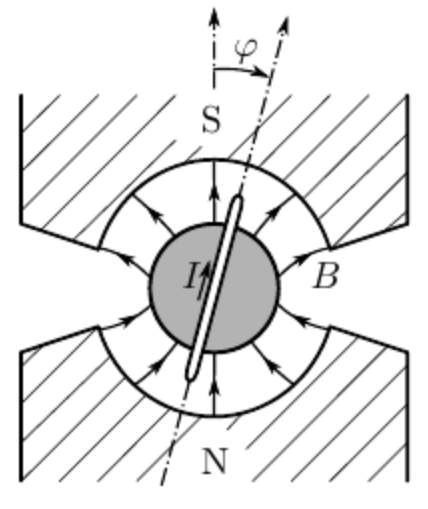
\includegraphics[width=1\textwidth]{3.2.6_1.png}
    \textbf{Рис. 1.} Рамка с током в магнитном поле
\end{center}
\end{wrapfigure}

\hfill \break Главной частью баллистического гальванометра является подвешенная на вертикальной нити рамка, помещенная в поле постоянного магнита. Вырез цилиндрической формы в полюсах магнита и ферромагнитный цилиндр на оси системы делают поле в зазоре радиальным (рис. 1). Скрепленное с рамкой зеркальце служит для измерения угла поворота рамки. К рамке прикреплен полый цилиндр, который сильно увеличивает момент инерции и, следовательно, период колебаний подвижной системы, не очень ее утяжеляя.

\hfill \break Баллистический гальванометр позволяет измерять как постоянный ток (\textit{стационарный} режим), так и заряд, протекший через рамку за некоторое время (\textit{баллистический} режим). В баллистическом режиме гальванометр может работать, если время протекания заряда много меньше периода собственных колебаний подвижной рамки. Поэтому период колебаний делают большим (5-15 с).

\subsection{Уравнение движения рамки в магнитном поле}
\hfill \break На помещенную в магнитное поле рамку гальванометра, по которой течет ток, действуют момент сил закрученной нити, момент сил трения и момент магнитных сил.

\hfill \break Механический момент упругих сил нити:

\begin{equation}\label{ linkname }
M_{1} = -D\varphi,
\end{equation}

\hfill \break где $D$ $-$ модуль кручения нити, а $\varphi$ $-$ угол поворота рамки от положения равновесия.

\hfill \break Момент сил вязкого трения:

\begin{equation}\label{ linkname }
M_{2} = -\beta_\text{тр}\dot\varphi.
\end{equation}

\begin{wrapfigure}{l}{0.3\textwidth}
\begin{center}
    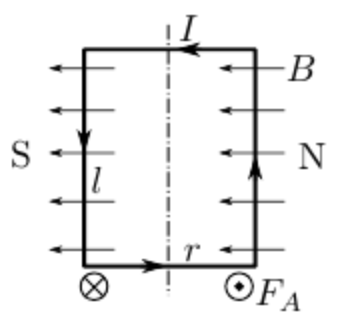
\includegraphics[width=1\textwidth]{3.2.6_2.png}
    \textbf{Рис. 2.} Силы Ампера, действующие на рамку в магнитном поле
\end{center}
\end{wrapfigure}

\hfill \break Пусть прямоугольная рамка с числом витков $N$, обтекаемая по контуру током $I_{\Sigma}$, помещена в магнитное поле с постоянной индукцией $B$ (рис. 2). Тогда на каждую боковую сторону рамки действуют силы $F_{A} = lNBI_{\Sigma}$, где $l$ $-$ длина стороны. Обозначив через $r$ расстояние от боковой стороны до оси вращения, найдем момент пары сил:

\begin{equation}\label{ linkname }
M_{3} = 2rlBNI_{\Sigma} = BSNI_{\Sigma},
\end{equation}

\hfill \break где $S = 2rl$ $-$ площадь одного витка рамки. В рамке, движущейся в магнитном поле с угловой скоростью $\dot\varphi$, наводится ЭДС индукции:

\begin{equation}\label{ linkname }
\varepsilon = -\frac{d\Phi}{dt} = -BSN\dot\varphi,
\end{equation}

\hfill \break где $\frac{d\Phi}{dt}$ $-$ скорость изменения магнитного потока, пронизывающего рамку. Пренебрегая самоиндукцией рамки, можно считать, что эта ЭДС вызывает индукционный ток:

\begin{equation}\label{ linkname }
I_\text{инд} = \frac{\varepsilon_\text{инд}}{R_{\Sigma}},
\end{equation}

\hfill \break где $R_{\Sigma} = R_{0} + R$ $-$ полное сопротивление цепи, состоящее из сопротивления рамки $R_{0}$ и сопротивления внешнего участка цепи $R$. Связанный с ЭДС индукции момент всегда тормозит вращение рамки:

\begin{equation}\label{ linkname }
M_{3} = M_\text{инд} = BSNI_\text{инд} = -\frac{(BSN)^2}{R_{\Sigma}}\dot\varphi.
\end{equation}

\hfill \break Этот момент значительно превосходит момент сил трения рамки, поэтому далее можем пренебречь $M_{2}$. Суммарный ток в рамке определяется ЭДС индукции и некоторым сторонним источником ЭДС:

\begin{equation}\label{ linkname }
I_{\Sigma} = \frac{\varepsilon + \varepsilon_\text{инд}}{R_{\Sigma}} = I + I_\text{инд}.
\end{equation}

\hfill \break Вращение рамки описывается уравнением моментов 

\begin{equation}\label{ linkname }
J\ddot\varphi = M_{\Sigma},
\end{equation}

\hfill \break где $J$ $-$ момент инерции подвижной системы. Тогда эту формулу можно представить в виде:

\begin{equation}\label{ linkname }
\ddot \varphi + 2\gamma\dot\varphi + \omega_{0}^2\varphi = KI.
\end{equation}

\hfill \break Здесь параметры $\gamma, \omega_{0}$ колебательной системы и коэффициент $K$ связаны с параметрами гальванометра формулами:

\begin{equation}\label{ linkname }
K = \frac{BNS}{J}; \space 2\gamma = \beta_\text{тр} + \frac{(BSN)^2}{JR_{\Sigma}} \approx \frac{(BSN)^2}{JR_{\Sigma}}; \space \omega_{0}^2 = \frac{D}{J}.
\end{equation}

\subsection{Режим измерения постоянного тока}
\hfill \break Если через рамку пропускать постоянный электрический ток, то заменой переменной $\tilde{\varphi} = \varphi - KI/\omega_{0}^2$ уравнение (9) приводится к однородному уравнению, описывающему свободные затухающие колебания. Если подождать достаточно долго, чтобы собственные колебания затухли, в уравнении (9) можно положить $\dot \varphi = \ddot \varphi = 0$, так что

\begin{equation}\label{ linkname }
\varphi = \frac{K}{\omega_{0}^2}I = \frac{BSN}{D}I = S_{I}I = \frac{I}{C_{I}},
\end{equation}

\hfill \break где $S_{I} = \varphi/I = BSN/D$ называется \textit{\textbf{чувствительностью}} гальванометра к току, а обратная ей величина $C_{I} = 1/S{I} = D/(BSN)$ $-$ \textit{\textbf{динамической постоянной}} гальванометра. 

\subsection{Свободные колебания рамки}
\hfill \break Рассмотрим свободное движение рамки, то есть движение в отсутствие внешних источников, когда $I = 0$. В этом случае уравнение (9) примет вид

\begin{equation}\label{ linkname }
\ddot \varphi + 2\gamma\dot\varphi + \omega_{0}^2\varphi = 0.
\end{equation}

\hfill \break Возможные случаи движения рамки:

\begin{enumerate}
    \item{$\gamma < \omega_{0}$ (колебательный режим). В этом случае движение рамки носит колебательный характер и затухает со временем; а при малом затухании движение рамки близко к синусоидальному.}
    \item {$\gamma = \omega_{0}$ (критический режим). Этот режим реализуется при сопротивлении внешнего участка цепи $R$, равном \textit{критическому} сопротивлению: $R_\text{кр} = \frac{(BSN)^2}{2\sqrt{DJ}} - R_{0}$. Движение при этом не имеет колебательного характера: отклоненная после начального толчка подвижная система плавно и экспоненциально возвращается к нулю:

    $$
    \varphi(t) = \dot\varphi_{0}te^{-\gamma t}
    $$}

    \item{$\gamma > \omega_{0}$ (затухание велико $-$ переуспокоенный гальванометр). Движение апериодическое, однако подвижная система приближается к равновесию медленнее, чем в критическом режиме.}
\end{enumerate}

\subsection{Режим измерения заряда}
\hfill \break Если пропустить через рамку короткий импульс тока, то можно считать, что весь ток успевает пройти при неотклоненном положении рамки. Рамка при этом получает толчок, в результате которого возникает движение, описываемое уравнением свободных колебаний (12). 

\hfill \break Величина $C_{q} = q/\varphi_{max}$ называется \textit{\textbf{баллистической постоянной}} гальванометра. Величина $S_{q} = 1/C_{q}$ называется \textit{\textbf{чувствительностью}} гальванометра к заряду. 

\hfill \break Максимальный отброс достигается при полном отсутствии затухания, однако в этом случае возникшие колебания рамки долго не смогут успокоиться. Тогда удобнее всего работать в режиме, близком к критическому, так как обеспечивается быстрое затухание колебаний и чувствительность прибора велика:

\begin{equation}\label{ linkname }
\varphi_\text{max, кр} = \frac{Kq}{\omega_{0}e}.
\end{equation}

\section{Экспериментальная установка}
\subsection{Определение динамической постоянной гальванометра}
\hfill \break Схема для исследования гальванометра в стационарном режиме представлена на рис. 3. Постоянное напряжение $U$ снимается с блока питания и измеряется вольтметром $V$. Ключ $K_{3}$ позволяет менять направление тока через гальванометр Г, делитель напряжения $-$ менять величину тока в широких пределах. Ключ $K_{2}$ служит для включения гальванометра, кнопка $K_{1}$ $-$ для его успокоения. Магазин сопротивлений $R$ позволяет менять режим работы гальванометра от колебательного до периодического.

\hfill \break Сила тока, протекающего через гальванометр, может быть вычислена как

\begin{equation}\label{ linkname }
I = \frac{R_{1}}{R_{2}} \frac{U_{0}}{R + R_{0}},
\end{equation}

\hfill \break где $U_{0}$ $-$ показание вольтметра, $R_{1}/R_{2}$ $-$ положение делителя, $R$ $-$ сопротивление магазина, $R_{0}$ $-$ внутреннее сопротивление гальванометра. 

\begin{center}
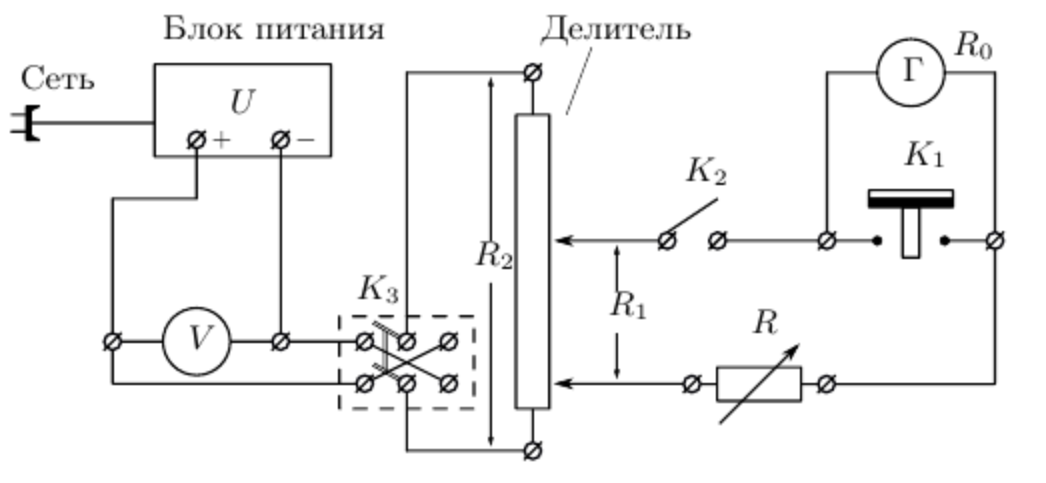
\includegraphics[width=0.65\linewidth]{3.2.6_3.png}\\
\textbf{Рис. 3.} Схема установки для работы гальванометра в стационарном режиме\\
\end{center}

\hfill \break Угол отклонения рамки от положения рановесия измеряется с помощью осветителя, зеркальца на рамке и шкалы, на которую отбрасывается луч света от зеркальца. Координата $x$ светового пятна на шкале

$$
x = a \cdot \arctan{2\varphi},
$$

\hfill \break где $a$ $-$ расстояние от шкалы до зеркальца. При малых углах $\varphi = x/(2a)$, тогда \textbf{динамическая постоянная}:

\begin{equation}\label{ linkname }
C_{I} = \frac{I}{\varphi} = \frac{2aI}{x}.
\end{equation}

\subsection{Определение критического сопротивления гальванометра}
\hfill \break Измерение критического сопротивления гальванометра можно выполнить при помощи той же схемы (рис. 3). С уменьшением R затухание колебаний увеличивается и колебательный режим переходит в апериодический. Условие ($\gamma = \omega_{0}$) можно представить как переходный между колебательным и апериодическим режимами. Воспользуемся логарифмическим декрементом затухания:

\begin{equation}\label{ linkname }
\theta = \ln{\frac{x_{n}}{x_{n+1}}},
\end{equation}

\hfill \break где $x_{n}$ и $x_{n+1}$ $-$ два последовательных отклонения колеблющейся величины в одну сторону. Измеряя зависимость $\theta (R)$, можно найти \textbf{критическое сопротивление} как параметр зависимости, которая следует из соотношения:

\begin{equation}\label{ linkname }
R_\text{кр} = \frac{R+R_{0}}{\sqrt{(\frac{2\pi}{\theta})^2+1}}-R_{0}.
\end{equation}

\subsection{Определение баллистической постоянной и критического сопротивления гальванометра, работающего в баллистическом режиме}
\hfill \break Для изучения баллистического режима работы гальванометра используется экспериментальная установка, представленная на рисунке 4. Система ключей устроена так, что нормально ключ $K_{2}$ замкнут, а ключи $K_{3}$ и $K_{4}$ разомкнуты. При нажатии на кнопку $K_{0}$ сначала размыкается ключ $K_{2}$, затем ключи $K_{3}$ и $K_{4}$. При нормальном положении $K_{0}$ конденсатор $C$ заряжается до напряжения $U_{C} = \frac{R_{1}}{R_{2}}U_{0}$ и получает заряд $q = CU_{C}$. При нажатии на $K_{0}$ конденсатор отключается от источника постоянного напряжения и подключается к гальванометру.

\begin{center}
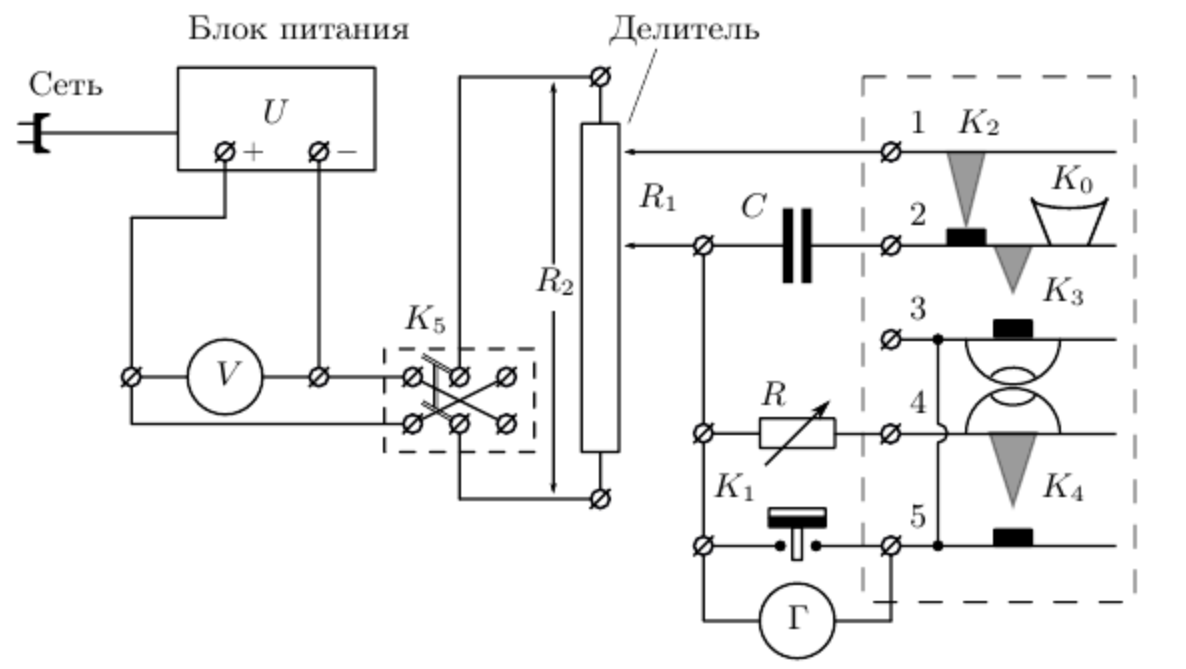
\includegraphics[width=0.65\linewidth]{3.2.6_4.png}\\
\textbf{Рис. 4.} Схема установки для работы гальванометра в баллистическом режиме\\
\end{center}

\hfill \break Емкость конденсатора подобрана так, что к моменту замыкания ключа $K_{4}$ весь заряд успевает пройти через гальванометр и рамка получает начальную скорость $\dot\varphi(\tau)$. Величину максимального отклонения рамки баз затухания можно рассчитать, если при разомкнутой цепи измерить реальное максимальное отклонение рамки $\varphi_{0}$ и логарифмический декремент затухания $\theta_{0}$. Тогда:

\begin{equation}\label{ linkname }
\varphi_{max} = \varphi_{0}e^{\theta_{0}/4} \approx \varphi(1 + \frac{\theta_{0}}{4})
\end{equation}

\hfill \break \textbf{Баллистическая постоянная} определяется соотношением:

\begin{equation}\label{ linkname }
C_{q} = \frac{q}{\varphi_{max}} = 2a\frac{R_{1}}{R_{2}}\frac{CU_{0}}{x_{max}},
\end{equation}

\hfill \break где $x_{max}$ $-$ величина первого отброса в критическом режиме, выраженная в делениях шкалы (мм).

\section{Ход работы}
\subsection{Определение динамической постоянной}
\hfill \break Подготовимся к работе: настроим осветитель гальванометра, соберем электрическую цепь согласно рисунку 3 и включим осветитель гальванометра. Установим делитель напряжения $\frac{R_{1}}{R_{2}} \approx \frac{1}{2000}$. Увеличивая сопротивление магазина, но не меняя делителя, снимем зависимость отклонения зайчика $x$ от сопротивления магазина $R$ и занесем результаты в таблицу. Ток в цепи рассчитаем по формуле (14). Зависимость тока в цепи от отклонения зайчика отобразим на графике (рис. 5):

\begin{center}
\begin{tabular}{|c|c|c|c|c|}\hline
$ R $, кОм & $ x $, см & $ \sigma_x $, см & $ I $, нА & $ \sigma_I $, нА\\\hline
8 & 22.7 & 0.1 & 88.24 & 0.39 \\\hline
10 & 18.5 & 0.1 & 71.43 & 0.39 \\\hline
12 & 15.7 & 0.1 & 60.00 & 0.38 \\\hline
14 & 13.7 & 0.1 & 51.72 & 0.38 \\\hline
16 & 12.1 & 0.1 & 45.45 & 0.38 \\\hline
18 & 10.8 & 0.1 & 40.54 & 0.38 \\\hline
20 & 9.9 & 0.1 & 36.59 & 0.37 \\\hline
30 & 6.9 & 0.1 & 24.59 & 0.36 \\\hline
40 & 5.4 & 0.1 & 18.52 & 0.34 \\\hline
50 & 4.5 & 0.1 & 14.85 & 0.33 \\\hline
\end{tabular} \\
\hfill \break \textbf {Таблица 1.} Зависимость отклонения зайчика от сопротивления, постоянный ток\\
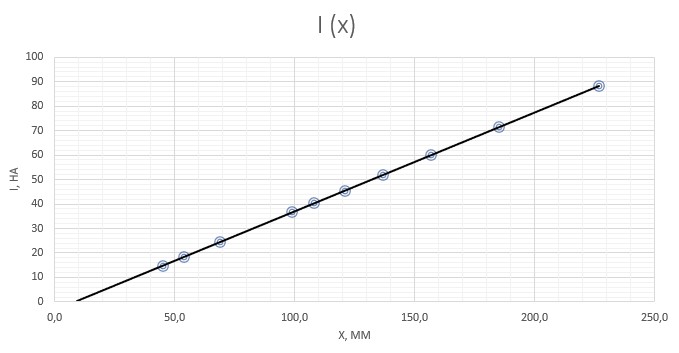
\includegraphics[width=0.95\textwidth]{3.2.6_5.png}\\
\textbf{Рис. 5.} График зависимости тока в цепи от отклонения зайчика\\
\end{center}

\hfill \break По графику при помощи МНК определим коэффициент наклона полученной кривой $k$ и свободный член $b$, а также погрешности их определения:

\begin{center}
\begin{tabular}{|c|c|}\hline
$ k $ & $ 0.403 \pm 0.007 $\\\hline
$ b $ & $ -3.258 \pm 0.010 $\\\hline
\end{tabular} \\
\hfill \break \textbf {Таблица 2.} Параметры графика зависимости тока в цепи от отклонения зайчика\\
\end{center}

\hfill \break Занесем в таблицу 3 некоторые параметры установки: $U_{0}$ $-$ показание вольтметра, $R_{2}$, $\frac{R_{1}}{R_{2}}$ $-$ значение делителя, $R_{0}$ $-$ внутреннее сопротивление гальванометра.
 
\begin{center}
\begin{tabular}{|c|c|}\hline
$ U_{0}, $ В & $ 1.5 $\\\hline
$ R_{2}, $ кОм & $ 10 $\\\hline
$ R_{1}/R_{2} $ & $ 1/2000 $\\\hline
$ R_{0}, $ Ом & $ 500 $\\\hline
\end{tabular} \\
\hfill \break \textbf {Таблица 3.} Некоторые параметры установки\\
\end{center}

\hfill \break Определим расстояние от шкалы до зеркальца гальванометра $a = 120$см. Зная это расстояние, мы можем рассчитать значение \textbf{динамической постоянной} по формуле (15):

$$
C_{I} = \frac{2aI}{x} = 2a\frac{I}{x} = 2ak = (0.97 \pm 0.02) \cdot 10^{-9} \frac{\text{А}}{\text{мм}/\text{м}}
$$

\hfill \break и, следовательно, \textbf{чувствительность гальванометра} к току:

$$
S_{I} = 1/C_{I} = (1.03 \pm 0.02) \cdot 10^9 \frac{\text{мм}/\text{м}}{\text{А}}.
$$

\subsection{Определение критического сопротивления}
\hfill \break Установим значение $R$, при котором зайчик отклоняется практически на всю шкалу, и разомкнем ключ $K_{2}$, чтобы обеспечить свободные колебания. Измерим пары последовательных отклонений зайчика в одну сторону и рассчитаем логарифмический декремент затухания $\theta_0$ разомкнутого гальванометра по формуле (16). Данные занесем в таблицу 4:

\begin{center}
\begin{tabular}{|c|c|}\hline
$ x_{n}, $ см & $ \theta_{0} = \ln{\frac{x_{n}}{x_{n+1}}} $\\\hline
17.90 & 0.225 \\\hline
14.30 & 0.218 \\\hline
11.50 & 0.223 \\\hline
9.20 & 0.218 \\\hline
7.40 & 0.210 \\\hline
6.00 & 0.203 \\\hline
4.90 & 0.228 \\\hline
$3.90$ & $ $ \\\hline
\end{tabular} \\
\hfill \break \textbf {Таблица 4.} Данные для определения логарифмического декремента затухания\\
\end{center}

\hfill \break Отсюда $\theta_{0} \approx 0.218 \pm 0.009$. При $R = 8$ кОм измерим период $T_{0}$ свободных колебаний рамки, он получается приблизительно равен 5.6 с. Это сопротивление также является наибольшим сопротивлением магазина, при котором при замыкании ключа $K_{3}$ зайчик не переходит нулевую метку на шкале, следовательно, это сопротивление близко к \textbf{критическому}.

\hfill \break Теперь для расчета $\theta$ проведем измерения отклонений зайчика после размыкания ключа $K_{3}$, увеличивая сопротивление магазина от $R = 3R_\text{кр}$ до $R = 10R_\text{кр}$. Результаты занесем в таблицу 5. Также построим график зависимости $(R+R_{0})$ от $(\sqrt{(\frac{2\pi}{\theta})^2+1})$ для качественного определения $R_\text{кр}$.

\begin{center}
\begin{tabular}{|c|c|c|c|c|c|}\hline
$ R $, кОм & $ x_{n} $, см & $ x_{n+1} $, см & $ \theta $, нА & $ \sqrt{(\frac{2\pi}{\theta})^2+1} $ & $ R+R_{0} $, кОм\\\hline
25 & 14.3 & 2.0 & 1.97 & 3.35 & 25.5 \\\hline
29 & 12.1 & 2.1 & 1.75 & 3.72 & 29.5 \\\hline
33 & 10.8 & 2.3 & 1.55 & 4.18 & 33.5 \\\hline
37 & 9.8 & 2.4 & 1.41 & 4.57 & 37.5 \\\hline
41 & 9.1 & 2.5 & 1.29 & 4.96 & 41.5 \\\hline
46 & 7.9 & 2.5 & 1.15 & 5.55 & 46.5 \\\hline
50 & 7.4 & 2.6 & 1.05 & 6.09 & 50.5 \\\hline
57 & 5.7 & 2.2 & 0.95 & 6.67 & 57.5 \\\hline
83 & 4.7 & 2.4 & 0.67 & 9.40 & 83.5 \\\hline
\end{tabular} \\
\hfill \break \textbf {Таблица 5.} Расчеты и измерения для определения критического сопротивления\\
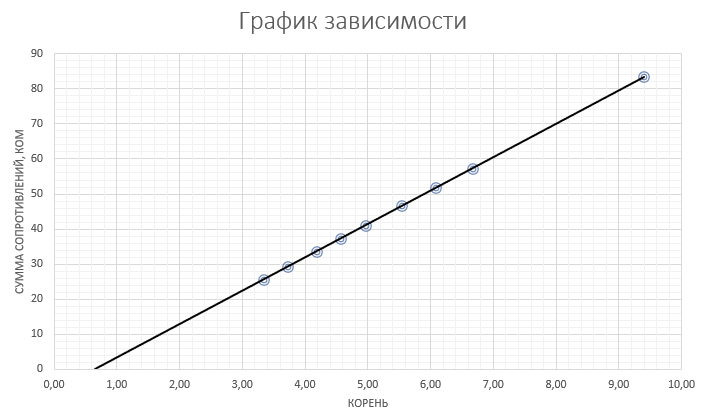
\includegraphics[width=0.95\textwidth]{3.2.6_6.png}\\
\textbf{Рис. 6.} График зависимости сопротивления в цепи от $ \sqrt{(\frac{2\pi}{\theta})^2+1} $\\
\end{center}

\hfill \break Определим коэффициент наклона построенного графика: $k = 9.52 \pm 0.19$. Тогда по формуле (17) определим значение \textbf{критического сопротивления}:

$$
R_\text{кр} = \frac{R+R_{0}}{\sqrt{(\frac{2\pi}{\theta})^2+1}}-R_{0} = k - R_{0} \approx (9.02 \pm 0.18) \text{кОм}.
$$

\subsection{Баллистический режим}
\hfill \break Соберем схему согласно рис. 4 и установим сопротивление магазина $R = 50$ кОм. Для измерения первого отброса зайчика разомкнем цепь, отсоеднив одну из клемм от магазина, и подберем делитель таким образом, чтобы при замыкании ключа $K_{0}$ первый отброс $x_{max}$ соответствовал отклонению зайчика почти на всю шкалу. Отброс 22.5 см (а это почти вся шкала) будет при значении делителя $1/70$. Тогда, по формуле (18), получим отброс в режиме свободных колебаний:

$$
x_{max} = x_{0}e^{\theta_{0}/4} = 22.5 \cdot e^{0.218/4} = 23.4 \text{см},
$$

\hfill \break а в критическом режиме первый оброс в $e$ раз меньше, чем в режиме свободных колебаний, поэтому

$$
x_\text{кр} = \frac{x_{max}}{e} \approx 8.6 \text{см}.
$$

\hfill \break Снова подключим магазин сопротивлений $R$ и будем уменьшать $R$ до тех пор, пока отброс не уменьшится до $1/3 - 1/4$ от своей начальной длины. Изобразим на графике на рис. 7 зависимость $x_{max}$ от $R+R_{0}$, необходимую для определения $R_{кр}$.

\begin{center}
\begin{tabular}{|c|c|}\hline
$ x_{max}, $ см & $ R + R_{0}, $ кОм\\\hline
18.5 & 50.5 \\\hline
17.3 & 40.5 \\\hline
16.5 & 30.5 \\\hline
14.4 & 20.5 \\\hline
11.1 & 10.5 \\\hline
9.5 & 8.5 \\\hline
8.3 & 6.5 \\\hline
6.6 & 4.5 \\\hline
4.0 & 2.5 \\\hline
2.6 & 1.5 \\\hline
\end{tabular} \\
\hfill \break \textbf {Таблица 6.} Зависимость максимального отброса от суммарного сопротивления\\
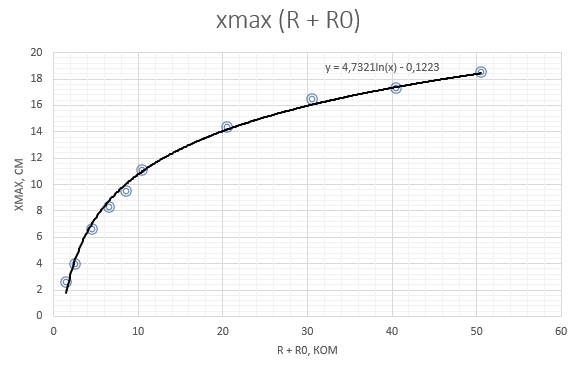
\includegraphics[width=0.95\textwidth]{3.2.6_7.png}\\
\textbf{Рис. 7.} График зависимости максимального отброса от суммарного сопротивления в цепи\\
\end{center}

\hfill \break Примерная формула, отображающая зависимость, показана на графике (рис. 7), где $x -> (R+R_{0})$. Из формул (18) и (13) мы знаем, что

$$
x_\text{max, кр} = \frac{Kq}{\omega_{0}e}
$$

\hfill \break и

$$
x_{max} = x_{0}e^{\theta_{0}/4} \approx x(1 + \frac{\theta_{0}}{4}).
$$

\hfill \break Тогда 

$$
x_\text{кр} = \ln{(R_\text{кр}+R_{0})^{4.7321}}-0,1223;
$$

$$
R_\text{кр} = e^{\frac{x_\text{кр}+0.1223}{4,7321}} - R_{0} = 5.92 \text{кОм}.
$$

\hfill \break По формуле (19) рассчитаем \textbf{баллистическую постоянную}, зная емкость конденсатора ($C = 2 \text{мкФ}$):

$$
C_{q} = 2a\frac{R_{1}}{R_{2}}\frac{CU_{0}}{x_\text{кр}} = 2 \cdot 1.20 \cdot \frac{1}{70} \cdot \frac{2 \cdot 10^{-6} \cdot 1.5}{86} = (1.19 \pm 0.01) \frac{\text{нКл}}{\text{мм}/\text{м}}.
$$

\hfill \break Тогда \textbf{чувствительность} гальванометра к заряду:

$$
S_{q} = 1/C_{q} = (0.84 \pm 0.01) \cdot 10^9 \frac{\text{мм}/\text{м}}{\text{Кл}}.
$$

\hfill \break Теперь определим время релаксации. Мы знаем, что к моменту замыкания ключа весь заряд должен успеть пройти через гальванометр, чтобы рамка приобрела некоторую скорость и начались колебания, поэтому время релаксации должно быть сильно меньше периода колебаний.

$$
\tau = R_{0}C = 1 \cdot 10^{-6} \text{с} \ll T_{0},
$$

\hfill \break следовательно, эксперимент верен.

\section{Вывод}
\hfill \break В данной лабораторной работе мы изучили работу гальванометра в стационарном и баллистическом режимах и определили ряд его характеристик. Так, была рассчитана динамическая постоянная:

$$
C_{I} = (0.97 \pm 0.02) \cdot 10^{-9} \frac{\text{А}}{\text{мм}/\text{м}},
$$

\hfill \break баллистическая постоянная:

$$
C_{q} = (1.19 \pm 0.01) \cdot 10^{-9} \frac{\text{Кл}}{\text{мм}/\text{м}},
$$

\hfill \break и было определено критическое сопротивление тремя разными способами:

\begin{center}
\begin{tabular}{|p{4cm}|p{4cm}|p{4cm}|}\hline
$ R_\text{кр}, $ кОм - подбор & $ R_\text{кр}, $ кОм - по графику в стационарном режиме & $ R_\text{кр}, $ кОм - по графику в баллистическом режиме \\\hline
8 & 9.02 & 5.92 \\\hline
\end{tabular} \\
\hfill \break \textbf {Таблица 7.} Результаты измерения критического сопротивления внешнего участка цепи тремя способами\\
\end{center}





























\end{document}
